% PARTES DEPOIS DO TEXTO
% Remova o % inicial de uma linha \input para ativar o item correspondente.
\postextual

% Geradas automaticamente a partir das citações e de bibliografia.bib.
%% Referências bibliográficas

% Não escreva referências aqui: cadastre as obras em bibliografia.bib.
%
% abntex-ifpi/abntex-ifpi.bib não contém obras: ele só carrega o perfil
% de citação da NBR 10520:2023. Mantenha-o na lista.
\bibliography{abntex-ifpi/abntex-ifpi,bibliografia}


% % Glossário manual: ative em estrutura/pos-textual.tex e substitua os termos.
\clearpage
\chapter*{Glossário}
\addcontentsline{toc}{chapter}{Glossário}
\begin{description}
  \item[Modelo] Estrutura inicial que pode ser adaptada ao trabalho.
  \item[Compilação] Processo que transforma os arquivos do projeto em PDF.
\end{description}
\clearpage


% Apêndice: material produzido por você. Comente se não for utilizar.
% APÊNDICES: materiais elaborados por você, como questionários e roteiros.
% Para retirar todos os apêndices, comente sua inclusão em estrutura/pos-textual.tex.
\begin{apendicesenv}
\renewcommand{\appendixtocname}{\texorpdfstring{\MakeUppercase{\apendicesname}}{\apendicesname}}

% Comente a linha seguinte para retirar a página de abertura dos apêndices.
\partapendices

% Cada \chapter cria um apêndice, com letra atribuída automaticamente.
% EXEMPLO -- apague este apêndice inteiro ou substitua seu conteúdo.
\chapter{Exemplo de apêndice}
\label{apendice:trabalhos}

Esta página é uma demonstração: o apêndice vem ativado para você ver como
ele aparece. Substitua o conteúdo por um material complementar produzido
na sua pesquisa (questionário, roteiro de entrevista, código-fonte) ou
desative o apêndice comentando a linha correspondente em
\texttt{estrutura/pos-textual.tex}.

\begin{table}[htb]
  \centering
  \ABNTEXfontereduzida
  \caption{Visão geral dos trabalhos selecionados: exemplo fictício}
  \label{tab:appendix-trabalhos-aprovados}
  \begin{tabularx}{\linewidth}{llX}
    \toprule
    \textbf{Identificador} & \textbf{Tipo} & \textbf{Descrição} \\
    \midrule
    S01 & Artigo & Síntese do primeiro trabalho selecionado. \\
    S02 & Dissertação & Síntese do segundo trabalho selecionado. \\
    \bottomrule
  \end{tabularx}
  \fonte{Elaboração própria.}
\end{table}
\end{apendicesenv}


% Anexo: material de terceiros. Verifique a fonte e a permissão de uso.
% % ANEXOS: materiais de terceiros, com a fonte e a permissão de uso verificadas.
% Ative este arquivo em estrutura/pos-textual.tex quando necessário.
\begin{anexosenv}
% Ative a linha seguinte se desejar uma página de abertura.
% \partanexos
% Substitua a imagem pelo documento pertinente à sua pesquisa.
\chapter{Trecho da carta de Pero Vaz de Caminha}
\label{anexo:a}

\begin{figure}[htb]
  \centering
  \caption{Documento ilustrativo fornecido com o modelo}
  \label{fig:carta}
  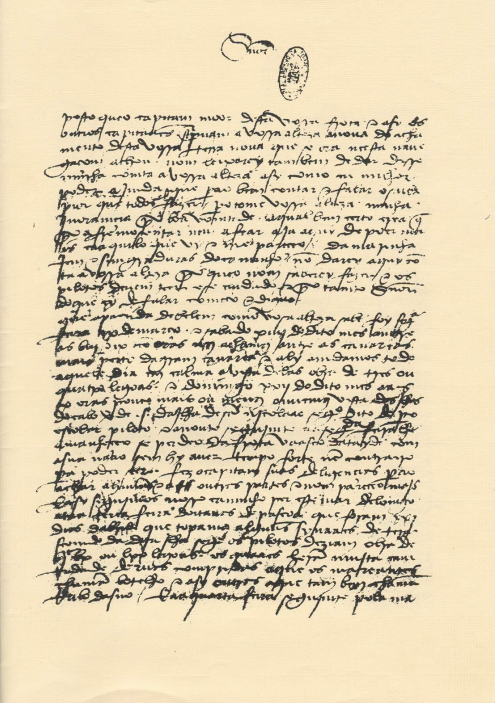
\includegraphics[width=0.9\linewidth,height=0.65\textheight,keepaspectratio]{imagens/carta_pero_vaz.png}
  \fonte{Arquivo do modelo original; confira a procedência antes de reutilizar.}
\end{figure}

\end{anexosenv}


% Índice remissivo: consulte a etapa MakeIndex em docs/guia-iniciante.md.
% % Ative \makeindex no preâmbulo e marque termos com \index{termo} no texto.
% Compile com latexmk, que executa MakeIndex quando necessário.
\phantompart
\printindex

% % Ative em estrutura/pos-textual.tex somente se a entrega incluir um CD.
\newpage
\thispagestyle{empty}
\begin{center}
\covers[{\vspace{1.5cm} \Large \MakeUppercase{Curso de \imprimirnomedocurso} \\ \vspace{1cm} \textbf{\imprimirautor} \\ \vspace{0.5cm} {TÍTULO: \imprimirtitulo}}]{
	{\vspace{1.5cm} 
\includegraphics[height=2cm]{abntex-ifpi/logo_ifpi.pdf} \\ \vspace{1cm} \MakeUppercase{Curso de \imprimirnomedocurso} \\ \vspace{1cm} {\textbf{\imprimirautor}} \\ \vspace{0.3cm} {TÍTULO: \imprimirtitulo} \\ \vspace{1.5cm} \MakeUppercase{\imprimirlocal} \par \imprimirdata}
}{
	\MakeUppercase{\tiny \imprimirtitulo}
}
\end{center}

